\documentclass[12pt]{article}
\usepackage[utf8]{inputenc}
\usepackage[T1]{fontenc}
\usepackage[english]{babel}
\usepackage{ifpdf,newtxtext,newtxmath} 
\usepackage{array,graphicx,dcolumn,multirow,hevea,abstract,hanging,fancyhdr}

\usepackage{graphicx}
\usepackage{dblfloatfix}    % To enable figures at the bottom of page
\usepackage[demo]{graphicx} % [demo] option for empty figure
\usepackage{kantlipsum}
% change next 3 lines each issue
\newcommand{\jref}{Advanced Multivariate Statistics}
\newcommand{\jhead}{Advanced Multivariate Statistics Course}
\newcommand{\jdate}{December 2020}
\topmargin=-.3in \oddsidemargin=.3in \evensidemargin=.3in \textheight=9in \textwidth=6in
\pagestyle{fancy} 
\fancyhead[L]{\protect\small \href{\jref}{\jhead}, \jdate}
\fancyhead[R]{\protect\small Advanced Cluster Analysis} % replace with running head
\fancypagestyle{firstpage}{%
 \lhead{\protect\small \href{\jref}{\jhead}, \jdate}
 \rhead{}
}
\usepackage[labelfont=sc,textfont=sf]{caption}
\usepackage[hyperfootnotes=false,breaklinks=true]{hyperref} % was dvipdfmx
% \usepackage[hyperfootnotes=false,breaklinks=true,linkbordercolor={1 1 1},citebordercolor={1 1 1}]{hyperref}
% \usepackage{natbib} % must come afer hyperfootnotes, use 2nd version for bibtex
% \setlength{\bibsep}{0pt}
\urlstyle{rm}
\usepackage[hyphenbreaks]{breakurl}
% DO NOT USE ADDITIONAL PACKAGES unless you make sure they work with Hevea.
% You may define new commands, but these may cause other troubles, so try to avoid it.

% FOR BIBTEX USERS (Bibtex is not recommended, but we can use it):
% \usepackage{natbib} % must come afer hypperref
% in references: \bibliographystyle{apalike3} \setlength{\bibsep}{0pt} \bibliography{WHATEVER}
% download http://journal.sjdm.org/apalike3.bst
\usepackage{booktabs} % \toprule \midrule \bottomrule \cmidrule(lr){a-b}
% define centered and ragged columns:
\newcolumntype{L}[1]{>{\raggedright\arraybackslash }p{#1}} % can use m{}
\newcolumntype{C}[1]{>{\centering\arraybackslash }p{#1}}
\newcolumntype{R}[1]{>{\raggedleft\arraybackslash }p{#1}}
\newcolumntype{d}[1]{D{.}{.}{#1}} % d{3.2} for 3 places on l, 2 on r
\newcommand{\mc}{\multicolumn}
\setlength\tabcolsep{1mm}
\setlength\columnsep{5mm}
\setlength\abovecaptionskip{1ex}
\setlength\belowcaptionskip{.5ex}
\setlength\belowbottomsep{.3ex}
\setlength\lightrulewidth{.04em}
\renewcommand\arraystretch{1.2}
\renewcommand{\topfraction}{1}
\renewcommand{\textfraction}{0}
\renewcommand{\floatpagefraction}{.9}
% \renewcommand{\baselinestretch}{1.00} \large\normalsize % for fixing spaces
\widowpenalty=1000
\clubpenalty=1000
\setlength{\parskip}{0ex}
\let\tempone\itemize
\let\temptwo\enditemize
\let\tempthree\enumerate
\let\tempfour\endenumerate
\renewenvironment{itemize}{\tempone\setlength{\itemsep}{0pt}}{\temptwo}
\renewenvironment{enumerate}{\tempthree\setlength{\itemsep}{0pt}}{\tempfour}

%%%%%%%%%%%%%%%%%%%%%%%%%%%%%%%%%%%%%%%%%%%%%%%%%%%%%%%%%%%%%%%%%%%%%
\setcounter{page}{1} % start with first page

\title{An application of clustering methods to cluster COVID-19 scholarly articles 
}

\author{
Quynh Anh Nguyen\thanks{Data Science and Economics Program, University of Milan. Email: quynh.nguyen@studenti.unimi.it.}\;\,\thanks{Github: jyanqa}
%\and 
 % Some O. Person\thanks{Yet another place.} 
}

\date{} % leave empty
\begin{document} % goes here

\begin{htmlonly}
\href{\jref}{\jhead}, \jdate, pp.\
\end{htmlonly}

\maketitle
\thispagestyle{firstpage}

\begin{abstract}

The main objectives of this project are clustering academic articles into different groups. The data set is CORD-19, resource of over 300,000 scholarly articles about COVID19 from the White House and a coalition of research groups. A subset of 1000 articles will be spitted from the original data to use in this project. Initially, each article from the data set will be parsed, cleaned and vectorized. Principle Component Analysis (PCA) will be subsequently applied on vectorized data to reduce the dimensions of the data. By then, K-Means and Gaussian Mixture Method are applied to cluster the projected data set. Last but not least, we find the representative keywords of each cluster and visualize them on the word-cloud plot. The result reveals that there are approximately 17 clusters by K-Means Method and 6 cluster by Gaussian Mixture Method. The clusters determined by K-Means surprisingly performed better than Gaussian Mixture Methods. Each cluster represents a distinctly COVID19-related concern such as International Law and Public Health Policy, Coronavirus and Schooling issue, Symptoms and Treatment and so on. 

\smallskip
\noindent
Keywords: GMM, K-Means, Model-based Method, NLP
\end{abstract}

%\saythanks

\setlength{\baselineskip}{16pt plus.2pt}

\section{Introduction}

 This project aims to cluster 1000 academic articles into different similarity groups and extract its main literature topics by applying NLP techniques, reducing dimensions of the data and comparing the results of two clustering methods, K-Means and Gaussian mixture model (GMM). Author wishes to contribute the fundamental statistical understanding to assist the medical community and researchers retrieve article references more convenient and efficient.
\section{Dataset}
CORD-19 is a resource of over 350,000 scholarly articles about COVID-19, SARS-CoV-2, and related corona viruses. 
The dataset is pre-processed by dropping duplicates articles, removing data points whose missing value and deleting articles that were published before 2019.  This is a huge data set , thus I am going to create a subset of 1000 articles after having preprocessed the original data set. Since the data set provides a lot of features of each article, I am going to extract the set of 4 features (paper id, title, abstract, body text) of each article. By using library \textit{langdetect}, a distribution of language using in 1000 articles is explored. All articles that are not in English are dropped, the data set now remains 966 articles. After that, the data will be converted text to lower case, removed punctuation and removed stop-words such as few, we, thru, etc. At the end of this data prepossessing step, we vectorized the body text of each article. The data frame now is converted into a matrix of  996 rows and 4096 predictors. 
\section{Method} % example of a heading
\paragraph{Principle Component Analysis }
The number of predictors in the data is much larger than the number of data-points. Therefore, PCA will be applied to our vectorized data to reduce the dimensions of the data. Dataset will be applied PCA in two ways. First, data will be reduced by finding the first PCs explain 95\% of variance. Thus, we avoid missing too much information from the original data. On the other hand, the dataset will be reduced into 2-dimensional data. This helps the visualization of the dataset be more convenient and intuitive. 
\subsection{Clustering analysis}
Clustering is an unsupervised method helps assign data objects into similar groups. Members of the same cluster must be similar and a member of one cluster must be as dissimilar as the members of others. In this project, we will examine the results after having applied two different Clustering methods. In detail, we will consider the number of clusters suggested by each method, the similarity of each cluster and the meaningful information extracted from clusters of each method.
\paragraph{Tuning the number of cluster}
As K is increasing, the within-cluster variation W always decreases; while the between-cluster variation B always increases. We will apply  Elbow and Gap Statistic method to define the optimal number of clusters. 

\subparagraph{Elbow}
The sum of squared distances from each point to its centroid is computed and plotted against k. There will be a k value after which decreases in distortion are minimal. The desired number of cluster is pointed out where the plot shows an ‘elbow’.

\subparagraph{Gap Statistics}
We compare the observed within-cluster variation $W(K)$ versus the within-cluster variation uniformly distributed data $W_{uniform} (K)$.
\begin{equation}
Gap(K) = \log W(K) - \log W_{uniform}(K)
\end{equation}

\paragraph{K-Means Method}
If centroids are $m_1, m_2, ... m_k$, and partitions are $c_1, c_2, ... c_k$, then one can show that K-Means converges to a {\it local} minimum of 
\[
\sum^K_{k=1} \sum_{i\in c_k} || x_i - m_k ||^2 \ \ \ \ \ \ \ \rm Euclidean \ distance
\]
Fitting K-Means algorithm: 
\begin{itemize}
\item Randomly determining the K centroids
\item Iterate until the cluster assignments stop changing 
    \subitem - For each of K clusters, compute the centroid, which is the p-length vector of the means in that cluster.
    \subitem - Assign each observation to the cluster whose centroid is closest using in Euclidean distance.
    \subitem This procedure is guaranteed to decrease the dissimilarity $W(K)$ at each step. 
\end{itemize}
\paragraph{Gaussian Mixture Method}
This is one of the most popular model-based clustering approaches available. The key idea behind model-based clustering is that the data are considered as coming from a mixture of underlying probability distributions. The most popular approach is the Gaussian mixture model (GMM) (Banfield and Raftery, 1993) where each observation is assumed to be distributed as one of k multivariate-normal distributions, where k is the number of clusters, commonly referred to as components in model-based clustering.
\paragraph{Evaluating the performance} K-Means or GMM clustered the articles but not extract its meaning. We will use LDA (Latent Dirichlet Allocation) to extract the most important terms of each cluster. In LDA, each document can be described by a distribution of topics and each topic can be described by a distribution of words. By checking the theme of extracted keywords, we can evaluate the good-fit result of clustering methods.

\section{Results}
\subsection{Tuning the number of cluster}
After reduced the dimension of our vectorized matrix by PCA method in which explain 95\% of variance, we have a new data including 966 data-points and 708 predictors. Before applying K-Means on this reduced data, we need to determine the optimal number of cluster. 
\begin{figure}[!tbp]
  \centering
  \begin{minipage}[b]{0.40\textwidth}
    \includegraphics[width=1\columnwidth]{2.eps}
    \caption{ Elbow method.}
  \end{minipage}
  \hfill
  \begin{minipage}[b]{0.40\textwidth}
    \includegraphics[width=1\columnwidth]{3gap.eps}
    \caption{ Gap Statistics method.\label{2}}
  \end{minipage}
\end{figure}

According to statistical folklore, the best K is located at the 'elbow' of the clusters inertia, within-cluster sum-of-squares criterion, while K increases. However, the Figure 1 does not demonstrate apparently the ‘elbow’. The optimal is determined in this case could be from 5 to 15 clusters. We can continue to find the optimal K by using Gap Statistics methods. 

The Figure \rep{2} shows the gap between the clusters inertia on the observed within-cluster variation $W(K)$ and the within-cluster variation of the reference data $W_{unif}(K)$. The optimal k is given by k for which the gap between the two results is maximum. According to Figure 2, the optimal k should be approximate 17 clusters.

\subsection{K-Means}

After determined the optimal number of cluster, we apply K-Means method. 

In fact, a good cluster model is the model that could maximize the similarity within-cluster and  minimize the similarity between-cluster. However, our data set is a $966\times708$ matrix, it is almost impossible to visualize to check whether the applied K-Means method well performed. Therefore, extracting keywords that represent for each cluster is an solution to examine the purity of these 17 clusters.

Figure 3 shows the keywords that are extracted from articles representing each cluster. The lexicon in the same group is pretty connected to each other and describes a certain topic. I have chosen some of 17 clusters and visualized them as word-cloud, figure 4. It is feasible to point out the Covid19-related concerns from these 6 clusters. They are treatments, business, guideline, authority policies, symptoms and education. 
\begin{figure*}[t!]
    \centering
    \includegraphics[width= 0.823\columnwidth]{4.17cluster.eps}
    \caption{Keywords of 11 clusters out of 17 clusters.}
\end{figure*}

\begin{figure*}[!b]
    \centering
    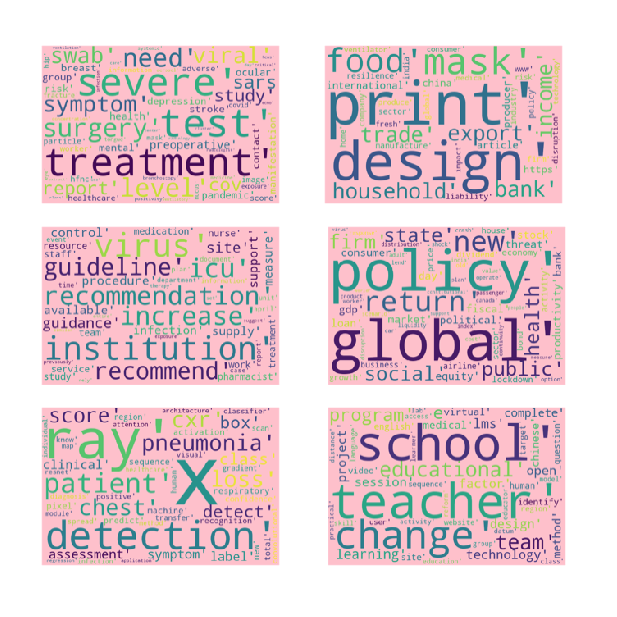
\includegraphics[width= 0.7\columnwidth]{5_cloud.eps}
    \caption{WordCloud of 6 clusters by K-Means method.}
\end{figure*}

\subsection{Gaussian Mixture Method}
In order to visualize the data point in a scatter plot, I reduced the original dataset, $966\times4096$ matrix, into a $966\times2$ matrix by PCA method. By using Elbow and Gap Statistic method as the previous steps, the optimal k is pointed out at 10 clusters. Figure 5 shows the scatter plot of reduced dataset applied K-Means method and the centroid of each cluster. K-Means finds suitable clustering result for well-separated data. For example, if we have simple binary large object of data, the K-Means algorithm can easily label those observations. As we can see in the figure 5, there appears to be a slightly overlap between clusters, such that we might not have complete confidence in the cluster assignment of points between them. 

\begin{figure}[!t]
  \centering
  \begin{minipage}[b]{0.45\textwidth}
    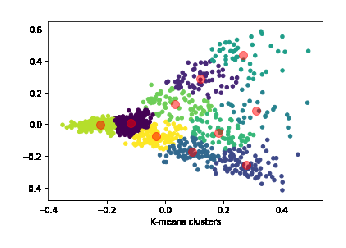
\includegraphics[width=1\columnwidth]{6_kmeans_2dim.eps}
    \caption{ K-Means Method.}
  \end{minipage}
  \hfill
  \begin{minipage}[b]{0.45\textwidth}
    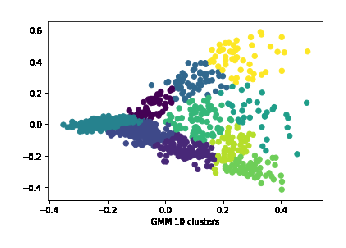
\includegraphics[width=1\columnwidth]{7_gmm_2dim.eps}
    \caption{Gaussian Mixture Method.\label{gmm}}
  \end{minipage}
\end{figure}
K-Means method lacks of flexibility in cluster shape and lack of probabilistic cluster assignment. This weakness is improved in Gaussian mixture model, one of the most popular model-based method. Figure 6 shows the scatter plot of the reduced 2-dimensional data set by choosing $k = 10$ as the having applied on K-Means method in figure 5. The 10 clusters in the figure 6 are  more robust than 10 clusters in the previous step. However, there is still the overlap parts between those clusters. In order to determine the optimal number of components for our model, we can consider AIC and BIC indicators.

Figure 7 reveals AIC and BIC index over the number of cluster. The optimal number of clusters is the value that minimizes the AIC or BIC. The AIC tells us that our test of 10 components above was not the best: either 7 or 8 components would have been a better option. Meanwhile, the BIC recommends 5 or 6 components for the model. Thus, we choose 6 components as a compromise. By assigning the optimal number of components to GMM model, the plot in Figure 8 shows us 6 clusters. These cluster are robust with respect to noise but there are less intersection compared to Figure 6, the plot when we applied GMM to 10 clusters.

%%%%%%%%%%%%%%%%%%%%%%%%%%%%%%
\begin{figure}[!b]
  \centering
  \begin{minipage}[b]{0.45\textwidth}
    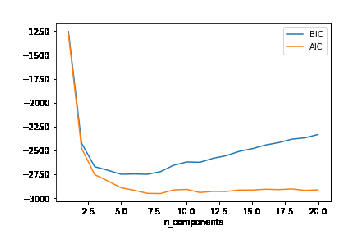
\includegraphics[width=1\columnwidth]{9_gmm_bic.eps}
    \caption{AIC and BIC index.}
  \end{minipage}
  \hfill
  \begin{minipage}[b]{0.45\textwidth}
    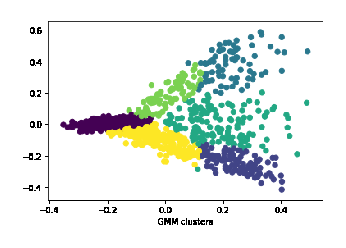
\includegraphics[width=1\columnwidth]{9_mm_scatterplot.eps}
    \caption{n\_component is 6.\label{nqa}}
  \end{minipage}
\end{figure}

%%%%%%%%%%%%%%%%%%%%%%%%%%%%%%%%%%%%%%%%%%%%%%%%%
\begin{figure}[!t]
  \centering
  \begin{minipage}[b]{1\textwidth}
    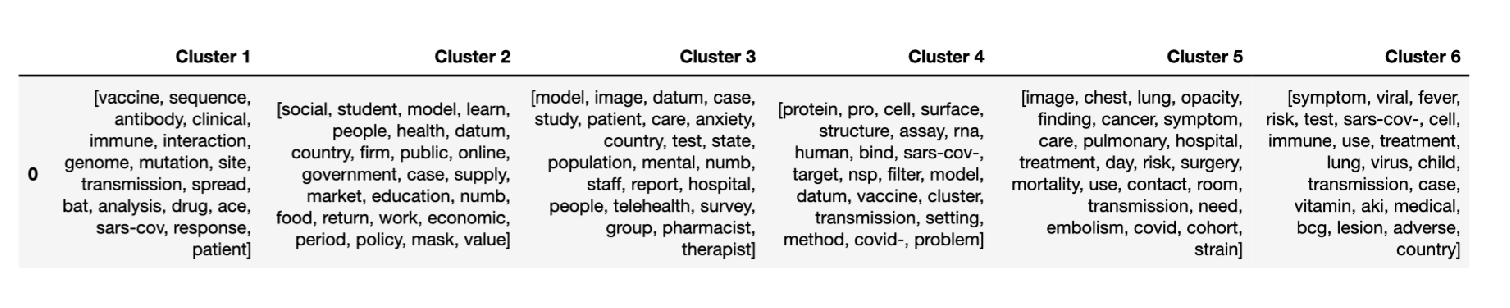
\includegraphics[width=1\columnwidth]{gmm_keywords.eps}
    \caption{Keywords of 6 clusters by GMM method.}
  \end{minipage}
  \hfill
  \begin{minipage}[b]{0.7\textwidth}
    \includegraphics[width=1\columnwidth]{gmmz0all.eps}
    \caption{WordCloud of 6 clusters by GMM method\label{nqa}}
  \end{minipage}
\end{figure}
%%%%%%%%%%%%%%%%%%

According to the scatter plots of 2-dimensional projected data in Figure 5 and Figure 8, the GMM prevails. But we will check whether this model-based method performed truly well. Based on GMM model, we assigned the label for each article, the label is one of 6 clusters. By then, the group of lexicon representing each group is drawn out. Figure 9 demonstrates the keywords retrieved from 6 clusters. Those keywords are plotted as word-cloud plot in Figure 10. It is undeniable that the keywords from GMM model are not as good as from K-Means model in term of describing a theme, which is our main objective of this project. 




%%%%%%%%%%%%%%%%%%%%%%%%%%%%%%%%%%%%%%
\section{Conclusion}


\begin{itemize}

    \item \textit{The optimal number of clusters of K-Means method are 10; whereas it is 6 for GMM model.} We can estimate the optimal k of K-Means method by Elbow method or Gap Statistics. Meanwhile, AIC and BIC are two indicators used to estimates the optimal components of the model-based method GMM.

    \item \textit{The GMM model shows the better result on two-dimensional data compared to K-Means method.} On this data set, after converted the original data to two-dimensional data, the clusters determined by GMM are more separated, less overlap compared to K-Means.

    \item \textit{In reality, the extracted keywords proved that K-Means is the better method.} Keywords of each clusters by K-Means model are describing a concrete content. Meanwhile, the keywords representing 6 clusters of GMM model are pretty confusing. This is one of the disadvantages of the Normal mixture models."The likelihood could be unbounded for the general normal mixture model and spurious solutions might emerge. Because,  several components form a single mode and observations are not assigned to the closest cluster due to different component-specific co-variance matrices."
    \item \textit{The different results of two methods can be explained by the dimension of the dataset, by the method determine the optimal cluster or components.} Applying PCA methods helps reducing dimensional of the data but we might lost a lot of information.  


\end{itemize}
% FOR BIBTEX USERS INSTEAD OF REFERENCES SECTION
%\bibliographystyle{apalike3}
%\bibliography{bibliography.bib}
% OR CAN ALSO INCLUDE THE BBL FILE AFTER THE NEXT LINE, INSTEAD OF THE LAST LINE
\section*{References}

\begin{hangparas}{1em}{1}

Manzi, G. (2020), Lecture 20: Course Recap, lecture notes. \textit{Advanced Multivariate Statistics B7416}, University of Milan, delivered December 2020.

 Boehmke, B. \& Greenwell, B. (2020).  Chapter 22 Model-based Clustering. \textit{Hands-On Machine Learning with R}, \url{https://bradleyboehmke.github.io/HOML/model-clustering.html}.
 
 VanderPlas, J. (2016).  In Depth: Gaussian Mixture Models.  \textit{Python Data Science Handbook}, \url{https://jakevdp.github.io/PythonDataScienceHandbook/05.12-gaussian-mixtures.html}.

 MaksimEkin (2020).  Loading data. \textit{COVID-19 Literature Clustering}, \url{https://www.kaggle.com/maksimeren/covid-19-literature-clustering/notebook}.
 
 Palafox, L. (2019).  A visual introduction to the Gap Statistics. \textit{The Glowing Python}, \url{https://glowingpython.blogspot.com/2019/01/a-visual-introduction-to-gap-statistics.html}.
 
\section*{Data Source}

The White House (2020).  Data set. \textit {CORD-19}, \url{https://www.kaggle.com/allen-institute-for-ai/CORD-19-research-challenge}.
\end{hangparas}

\end{document}
